
\begin{figure}[!htbp]\centering
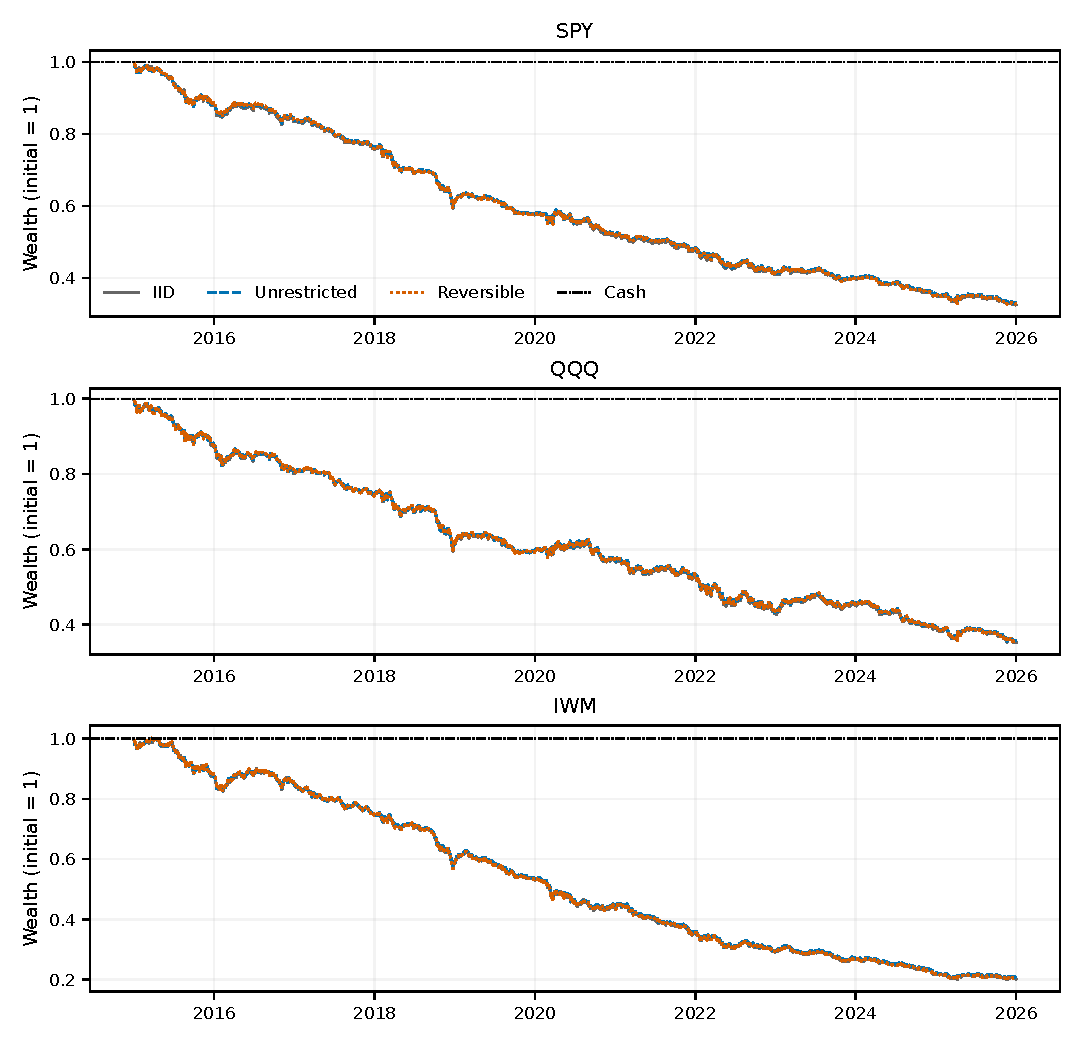
\includegraphics[width=\linewidth]{../figures/figure1.pdf}
\caption{Final-period net wealth at five basis points per side. Every model enters at the next open and liquidates at the close; cash earns zero. Overlapping curves indicate similar exposure, not equivalence of forecasts.}\label{fig:wealth}
\end{figure}

\begin{figure}[!htbp]\centering
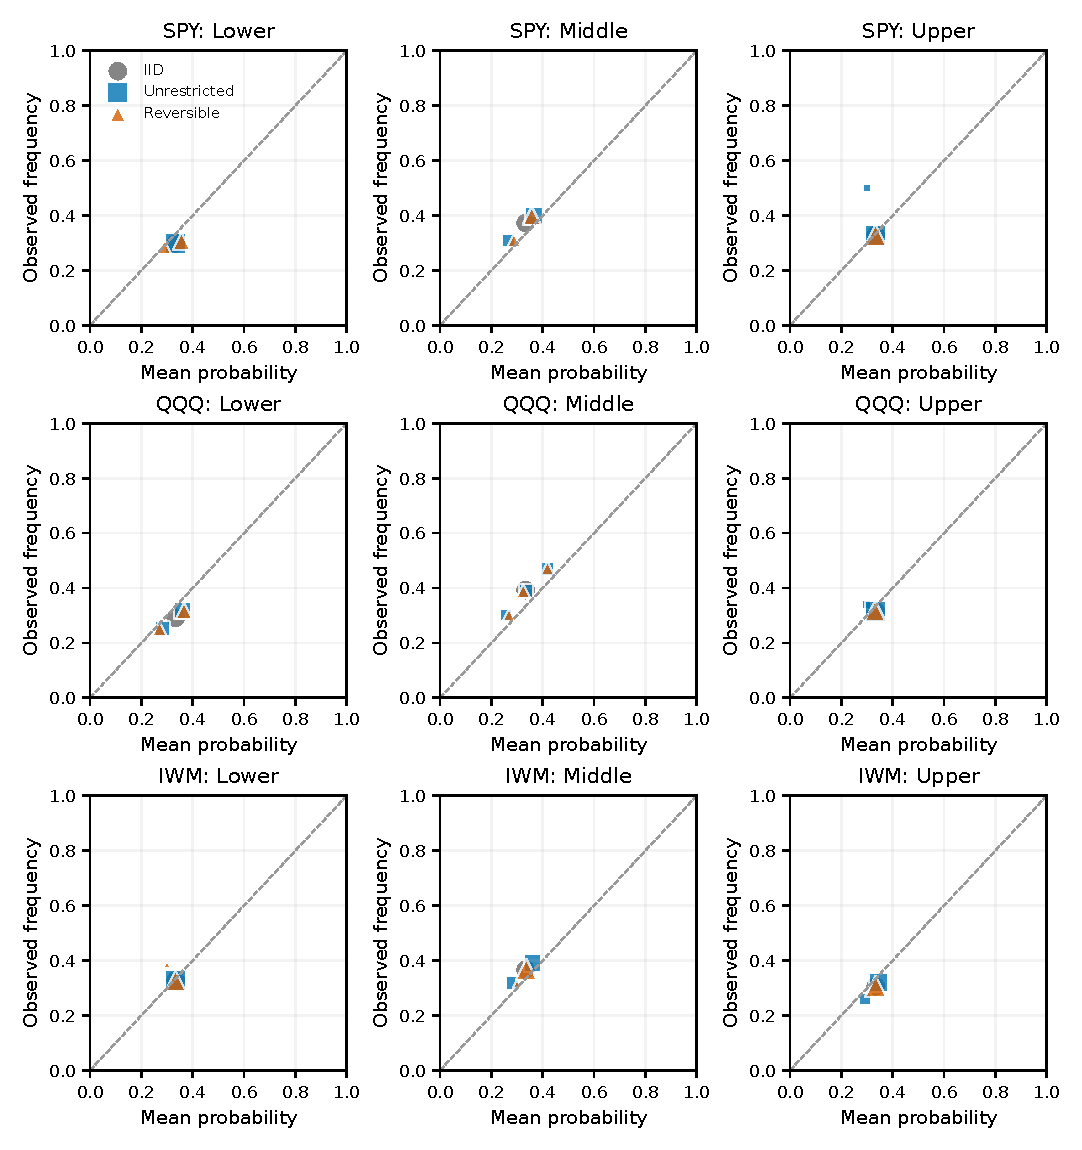
\includegraphics[width=\linewidth]{../figures/figure2.pdf}
\caption{Final-period class-wise calibration. Ten fixed bins are used; empty bins are omitted. Marker area increases with bin count. The diagonal denotes perfect bin-level reliability; sparse bins are descriptive. The common 0--1 axes retain the full probability scale; plotted points are bin averages, not individual forecast ranges. No confidence bands are shown here; a count-weighted summary and an independent-draw simulation diagnostic are reported in Appendix~\ref{app:families}.}\label{fig:calibration}
\end{figure}

\begin{figure}[!htbp]\centering
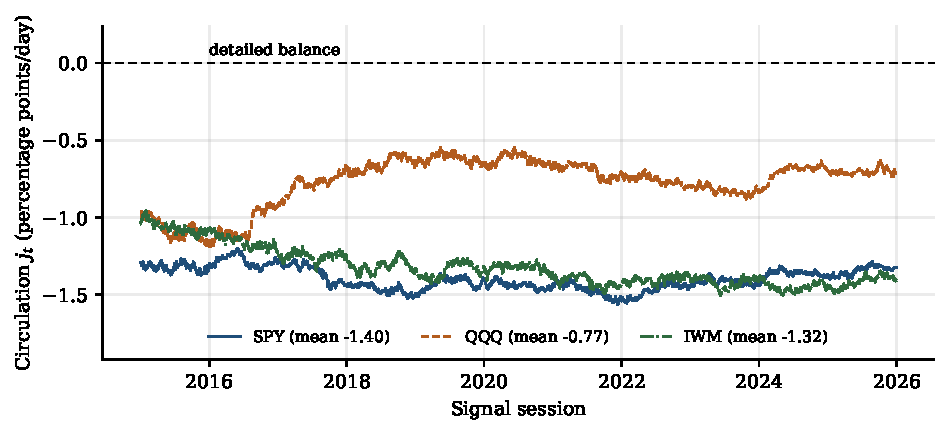
\includegraphics[width=0.88\linewidth]{../figures/figure5_circulation.pdf}
\caption{Fitted circulation $j_t=J_{12}=J_{23}=J_{31}$ of the unrestricted chain at each final-period origin, in percentage points of daily probability flow. The dashed line at zero is detailed balance, imposed by construction in the reversible fit. A negative value indicates net rotation in the direction Lower$\to$Upper$\to$Middle$\to$Lower. The plotted labels Down, Neutral and Up refer to relative terciles, not absolute return signs. The path is shown at the origin at which each forecast is formed; it is a property of the fitted transition matrix, not an additional observable.}
\label{fig:circulation}
\end{figure}

\begin{figure}[!htbp]\centering
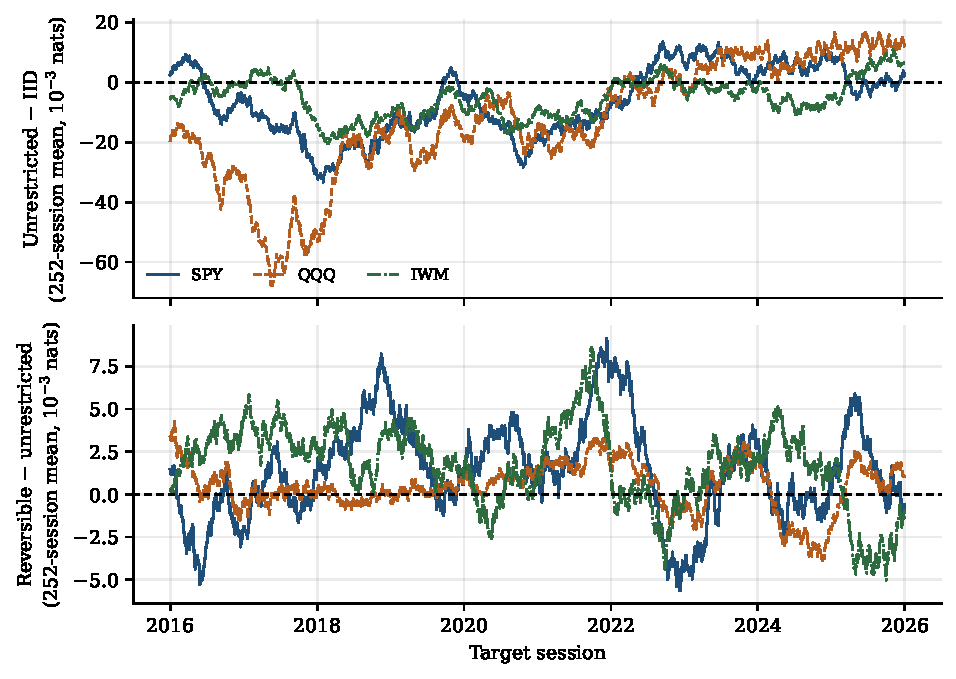
\includegraphics[width=0.88\linewidth]{../figures/figure6_rolling.pdf}
\caption{252-session rolling means of the two score differences, in $10^{-3}$ nats. Upper panel: unrestricted minus IID. Lower panel: reversible minus unrestricted. The zero line is no difference. Overlapping windows reuse almost all observations and the paths are descriptive; they show a larger unrestricted advantage early in the evaluation and deterioration in the later period, while the reversible difference stays mostly positive without a stable level.}
\label{fig:rolling}
\end{figure}
